\section{Структура ML проекта. Conda. DVC. Docker. Jenkins. DevOps практики. Хранилища секретов.}

\subsection*{Структура проекта}

\subsubsection*{project dir}
Локальная версия git репозитория;

Содержит в себе все файлы и метаданные проекта;

В большинстве случаев архив данной папки – дистрибутив
модели машинного обучения;

Имеет осмысленное название;

Внутри обязательно содержит конфигурацию репозитория –
папку .git;

В случае разработке на корпоративном устройстве/в облаке
необходима настроенная политика доступа RWX.

\subsubsection*{src}

Содержит весь исходный код проекта:
\begin{itemize}
    \item train.py – код взаимодействия с конфигурацией проекта
    (параметрами, путями к данным), содержит реализацию
    обучения модели, её сериализацию и логгирование;
    \item predict.py – код загрузки модели, вычисления метрик на
    предоставленных данных и сохранения результата;
    \item preprocess.py – код предварительной обработки данных,
    разбиения на тренировочную, тестовую и валидационную
    выборки;
    \item вспомогательные файлы (utils.py…) – код внешней логики
    взаимодействия со сторонними сервисами и любой другой
    код, необходимый для эксплуатации;
\end{itemize}

\subsubsection*{notebooks}

Хранит ноутбуки, описывающие анализ и выбор модели.

\subsubsection*{data}

\subsubsection*{experiments}

\subsubsection*{tests}

\subsection*{Conda}

\D{
    Conda - менеджер пакетов и система управления средой.
}

PIPvsConda:
\begin{itemize}
    \item Pip работает с python и пренебрегает зависимостями
    из не python библиотек. Работает с виртуальными средами
    python.
    \item Conda работает с виртуальными системными средами
    подходит для любого программного обеспечения.
\end{itemize}

\subsection*{DVC}

\D{
    DVC - инструмент для управления версиями моделей и
    данных.

    Работает совместно с git, используя его инфраструктуру.
    Создает метафайлы, описывающие жизненный цикл.
}

Помогает автоматизировать ML pipeline и отслеживать метрики,
поддерживать воспроизводимость.

\subsubsection*{Docker}

\D{
    Технология контейнеризации. Способ виртуализации ОС,
    при котором код, среда, библиотеки и зависимости
    упаковываются в единый контейнер.
}

Компоненты:
\begin{itemize}
    \item Клиент
    \item Хост
    \item Реестр
\end{itemize}

\begin{figure}[h]
	\centering
	\begin{minipage}[b]{0.8\textwidth}
		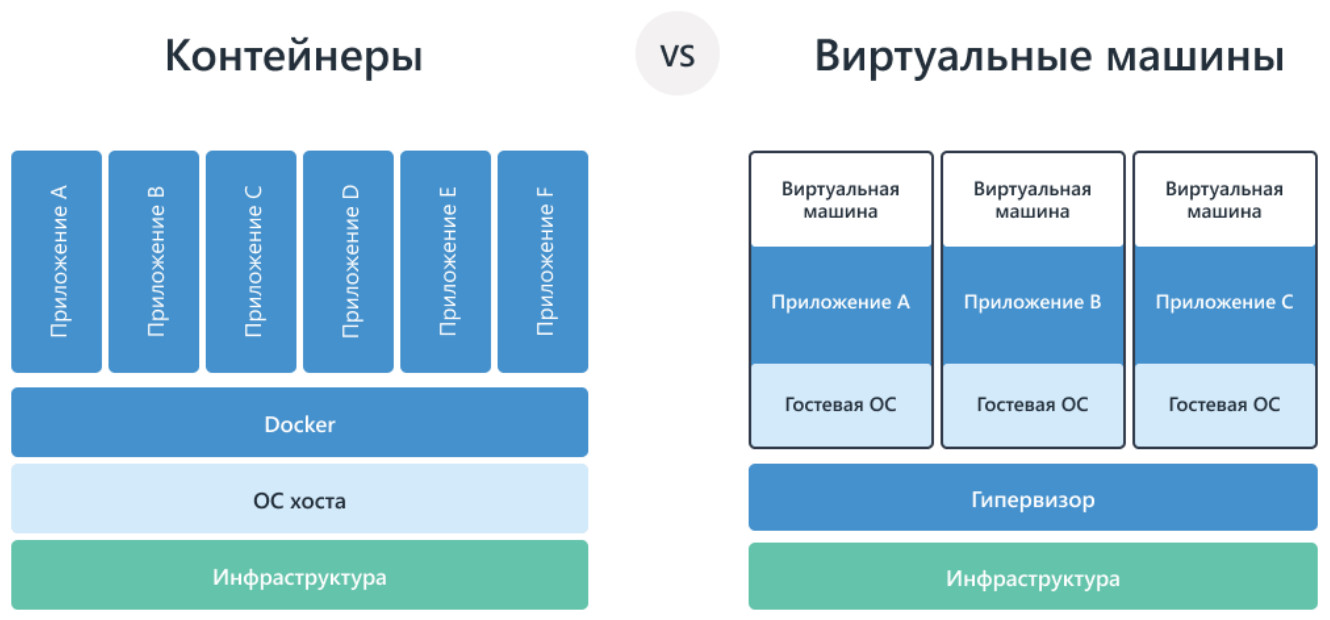
\includegraphics[width=\textwidth]{images/cvm.png}
	\end{minipage}
\end{figure}

\subsubsection*{Jenkins}

\D{
    CI. Предназначен для обеспечения процесса непрерывной
    интеграции программного обеспечения.
}

DevOpsLike:
\begin{itemize}
    \item CI - сборка
    \item CDL - CI + test
    \item CDP - CI/CD to prod
\end{itemize}